\documentclass{amsart}
\usepackage{amsmath,amsthm}
\usepackage{graphicx}
\usepackage{xcolor}
\usepackage{wrapfig}
\usepackage{url}
\usepackage{caption}
\usepackage{subcaption}
\usepackage[justification=centering]{caption}

\usepackage{algorithm} % Must be loaded *after* hyperref
\usepackage[noend]{algpseudocode}

\newtheorem{theorem}{Theorem}[section]
\newtheorem{lemma}[theorem]{Lemma}

\title{The dynamics of factored state hidden Markov models}
\date{1 December 2020}

\begin{document}

\maketitle

\section{Introduction and Notation}\label{sec:intro}

\subsection{Classical hidden Markov models}
In what follows we denote random variables with upper case Latin letters like 
$X$, the probability distributions from which they are drawn with calligraphy 
letters like $\mathcal X$ and specific values with lower case Latin letters like $x$.  Suppose we have a sequence of observations, 
\[
X_{1:T} := X_1,...,X_T
\]
where at each time $t$, the observation $X_t$ can be decomposed into its 
categorical and continuous components, that is 
\begin{eqnarray}\label{eqn:decomposition}
X_t = W_t\oplus V_t
\end{eqnarray}
where $W_{t}$ is drawn from the categorical space
\[ 
\mathcal W = \{1,...,D\}
\]
and $V_t$ is drawn from a $K$ dimensional Gaussian distribution, $\mathbb R^K$.
A hidden Markov model (HMM) is a latent state model that captures the Markov dynamics of a latent process underlying the observed data.  In its most basic form, the HMM models a sequence of hidden states
\[
Z_{1:T} := Z_1,...,Z_T
\]
corresponding to $X_{1:T}$, where for any time $t$, the hidden state $Z_t$ is 
drawn from the discrete\footnote{Hidden states can of course be drawn from more complicated probability 
distributions -- see, for example, Chapter 13 of Bishop's canonical text on the 
topic \cite{B06}.  For sake of brevity, this note will only 
consider the discrete hidden state space.} probability distribution
\[
\mathcal{Z} = \{h_1,...,h_N\}.
\]
The sequence of hidden states satisfy the {\em Markov property}, that is 
\[
p(Z_t\mid Z_{t-1})=p(Z_t\mid Z_{t-1},Z_{t-2},...,Z_1),
\]
and therefore form a Markov chain.  A fully parameterized HMM, denoted by 
$\Theta$, is given by a set of three probability distributions: the initial state probability, the transition probability and the 
emission probability.

For a given $\Theta$, we assume 
these three distributions have a fixed, parametric form given by 
\begin{eqnarray*}
p(Z_1=z) &=& p_1(z;\theta_1)\\
p(Z_t = z\mid Z_{t-1}=z') & = & p_z(z\mid z';\theta_z)\\
p(X_t=x\mid Z_t=z) & = &p_x(x\mid z;\theta_x),
\end{eqnarray*} 
where 
\[
\Theta = \{\theta_1,\theta_z,\theta_x\}.
\]
For $X_t$ as in equation (\ref{eqn:decomposition}) we can refine this further, 
by
\begin{eqnarray*}
p_x(x\mid z;\theta_x)& = &p_{cat}(w\mid z; \theta_{cat})\cdot p_{cont}(v\mid z; \theta_{cont})
\end{eqnarray*}
for
\begin{eqnarray*}
p(W_t=w\mid Z_t=z) & = & p_{cat}(w\mid z; \theta_{cat}),\\
p(V_t=v\mid Z_t=z) & = & p_{cont}(v\mid z; \theta_{cont}),
\end{eqnarray*}
with $\theta_x = \{\theta_{cat},\theta_{cont}\}$.
The $\theta_i$ will often be left off of the expressions above when is clear 
from context. 

The {\em initial state probability} given by $p_1$ is encoded in an $N\times 1$ 
vector describing the probabilty of inhabiting each of the $N$ hidden states at 
time $t=1$.  The $i^{th}$ term of the initial state vector is given by  
$p_1(h_i; \theta_1)$. 

The {\em transition probability}, which describes the 
likelihood of transitioning from any one state to another, is captured in an 
$N\times N$ matrix, 
\[
A=\begin{bmatrix}
a_{ij}
\end{bmatrix}_{i,j=1}^N \text{ where }a_{ij} = p_z(h_j\mid h_i;\theta_z)
\]
One relevant observation that we can make about the transition matrix, is that 
every row of $A$ necessarily sums to 1, since 
\begin{eqnarray}\label{eqn:transitionsum}
\sum_{j=1}^Np_z(h_j\mid h_i)=\sum_{j=1}^N\frac{p(h_j,h_i)}{p(h_i)}=1.
\end{eqnarray}
marginal over $h_i$.

The {\em emission probability} is the parameter that directly 
couples the observation sequence and the hidden 
state sequence and captures the probability of an observation vector given each 
of the hidden states. The categorical part of the emission probability can be 
described by a $D\times N$ matrix, 
\[
B = \left[b_{i}(d)\right]_{d,i=1}^{D,N}\text{ where }b_{i}(d) =p_{cat}(d\mid h_i; \theta_{cat}).
\]
For the continuous part of the emission probability, each hidden state, $h_i$ 
corresponds to a $K$-dimensional Gaussian distribution with a 
$K$-dimensional mean vector, $\mu_i$, 
and $K\times K$ covariance matrix, $\Sigma_i$ for each hidden state $h_i$, and 
hence 
\[
p_{cont}(v\mid 
h_i;\theta_{cont})=\frac{\exp\left(-\frac{1}{2}\left(v-\mu_i\right)\Sigma_i^{-1}\left(v-\mu_i\right)^T\right)}{\sqrt{(2\pi)^K\mid \Sigma_i\mid}}.
\]
The graphical model for a classical HMM can 
be seen in Figure \ref{fig:HMM}.  One primary goal in much of what follows, will be to learn the components of 
$\theta$.

\begin{figure}
\centering
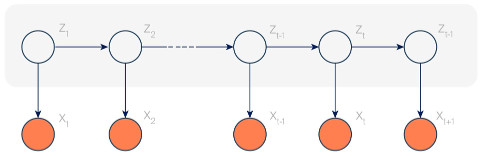
\includegraphics[scale=0.5]{figures/hmm.jpg}
\caption{The graphical model of a classical HMM}\label{fig:HMM}
\end{figure}

\subsection{Factored hidden Markov models}
In an fHMM with $M$ underlying Markov systems, the hidden state, $Z_t$, at time $t$, is an $M$-dimensional vector,
\[
Z_t = (Z_{t}^{(1)},...,Z_{t}^{(M)}),
\]
drawn from the probability distribution
\[
\mathcal Z = \mathcal{Z}^{(1)}\times ...\times \mathcal{Z}^{(M)}
\]
where 
\[
\mathcal Z^{(m)} = \{h_1^{(m)},...,h_{N_M}^{(m)}\}, 
\]
for all $1\leq m\leq M$.  To simplify the exposition, we will assume throughout this note that 
\[
N = N_1 = ...= N_M
\]
although a similar narrative will hold when this restiction is removed. 

The random variable $Z_t\in \mathcal Z$ can take on one of $N^M$ possible values, 
\begin{eqnarray}\label{eqn:vec}
s_i = (s_{i}^{(1)},...,s_{i}^{(M)})\text{ where }s_i^{(m)}\in \{h_1^{(m)},...,h_{N}^{(m)}\}
\end{eqnarray}
for $1\leq i\leq N^M$.  The set of hidden 
state variables in $\mathcal Z^{(m)}$ can be more concisely 
represented by a collection of $N$ 
many $N\times 1$ matrices, each 
of which is 0 in all but one component.  Therefore, we will represent the vector $s_i$ by a 
set of $M$ many $N\times1$ matrices corresponding to the appropriate 
$s_i^{(m)}$. A comprehensive treatment of fHMMs can be found in the foundational publication 
on the topic by Gharamani and Jordan \cite{GJ95}, but we will highlight some 
key components of that paper here.  

The initial state vector can take on one of $N^M$ values, therefore we will define the initial state probabilties by 
\[
\pi_{i_1,...,i_M} := p_1(\{h_{i_1}^{(1)},...,h_{i_M}^{(M)}\};\theta_1).
\] 
for any hidden state vector, subject to the restriction
\begin{eqnarray}\label{eqn:initialstate}
1 = \sum_{i_1=1}^N\cdots \sum_{i_M=1}^M \pi_{i_1,...,i_M}.
\end{eqnarray}
The transition probability will now be described by a collection of $M$ many $N\times N$ matrices, 
\[
\{A^{(1)},...,A^{(M)}\},
\]
where 
\[
A^{(m)} = \begin{bmatrix}
a_{ij}^{(m)}
\end{bmatrix}_{1\leq i,j\leq N}\text{ where } a_{ij}^m := p_z(h_j^{(m)}\mid 
h_i^{(m)}; \theta_z)
\]
for $1\leq m\leq M$, with the added restriction,
\begin{eqnarray}\label{eqn:transitionsum2}
1=\sum_{j=1}^Na_{ij}^{(m)}
\end{eqnarray}
which is just the fHMM analogue of equation (\ref{eqn:transitionsum}).

The probability of transitioning from one hidden state vector to another can 
then be constructed as a tensor product of these matrices.  More concretely, 
the probabilty of transitioning from a particular hidden state vector at time 
$t-1$ to any another hidden state vector at time $t$ can be decomposed as the product
\begin{eqnarray}\label{eqn:trans2}
p(Z_t\mid Z_{t-1}) = \prod_{m=1}^M p(Z_{t}^{(m)} \mid Z_{t-1}^{(m)}).
\end{eqnarray}
In this way each of the Markov processes evolves independently, according to 
its own dynamics. A graphical model for the fHMM can be seen in Figure 
\ref{fig:fHMM}.

\begin{figure}
\centering
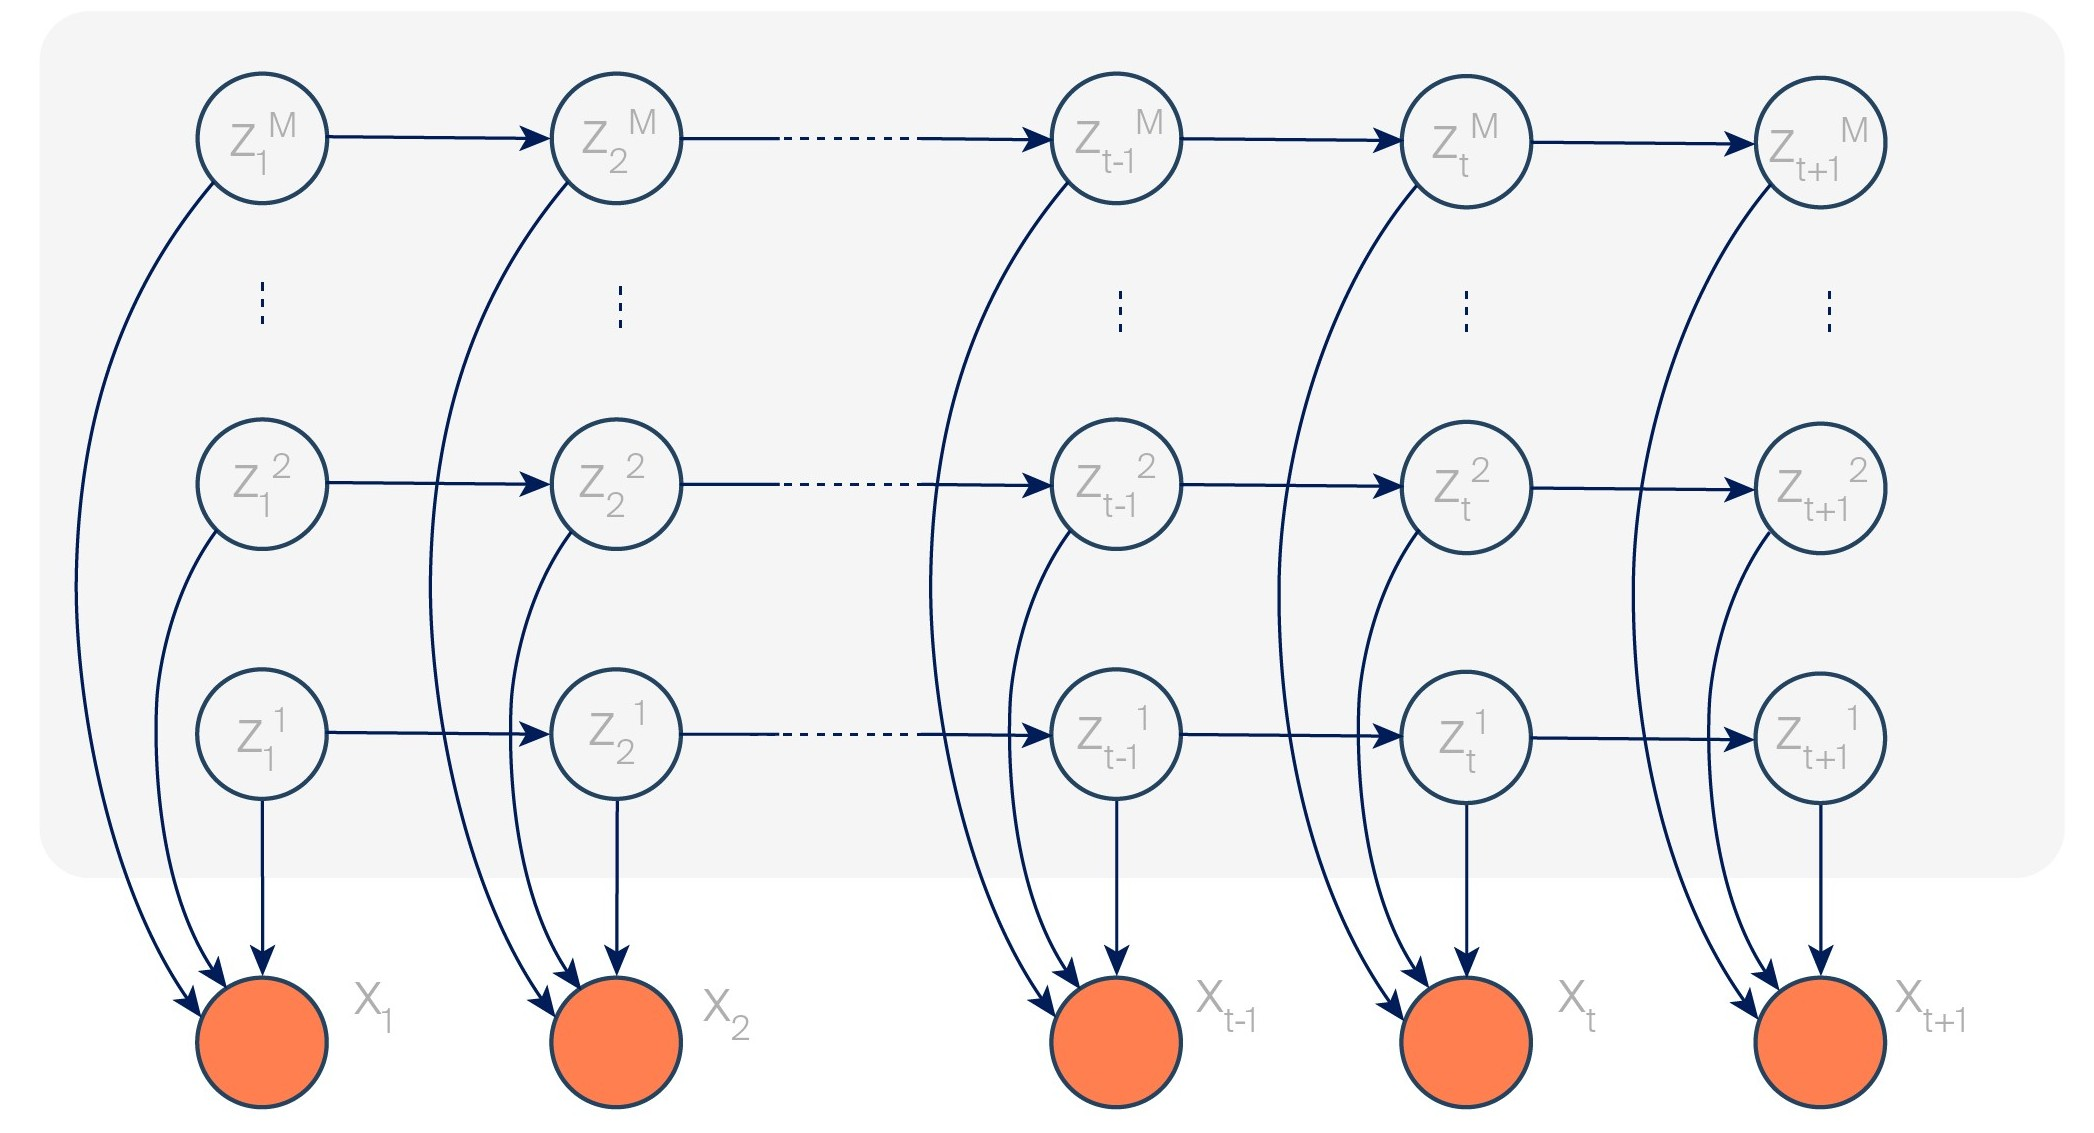
\includegraphics[scale=0.1]{figures/fhmm.jpg}
\caption{The graphical model of a factored HMM}\label{fig:fHMM}
\end{figure}

Although we want to maintain this marginal independence for the hidden states, 
$Z_{1:T}$, we would expect some dependence once we condition on the observation 
sequence, $X_{1:T}$.  To understand the intuition behind this, let's revisit our 
example of involving the five components of the wind turbine.  While we don't 
expect the status of the generator from time $t$ to $t+1$ to be connected to 
the status of the yaw motor from time $t$ to $t+1$, if we were to observe a 
power surge that causes the generator to experience a fault, that might 
increase the likelihood that the yaw motor experiences a fault\footnote{This is 
an example of what is known as ``Berkson's paradox".}.  If we consider 
the fHMM as a graphical model as in Figure (\ref{fig:fHMM}) we can couch this 
observation in the language of directed graphs and the so-called d-separation 
criterion. This conditional dependence means that, in particular, we would not expect the 
emission probability to decompose as a tensor product as in equation (\ref{eqn:trans2}). 

In the case of categorical observations we can 
describe the emission probability much like in the classical case, but encoding 
the information in a $D\times N^M$ matrix, $B$, where 
\[
B = \left[b_{i}(d)\right]_{d,i=1}^{D,N^M} \text{ where }b_{i}(d) = p_{cat}(d\mid 
s_i;\theta_{cat}).
\]
Since $s_i$ refers to the hidden state tuple
\[
s_i = (s_i^{(1)},...,s_i^{(M)}) \text{ where }s_i^{(m)} = h_{i_m}^{(m)}
\]
we will often refer to a single entry of the emission matrix as 
\[
b_{i}(d) = b_{i_1,...,i_M}(d)
\]
where no confusion will arise.  The situation becomes more complicated for continuous observations.  In 
particular, the mean values for each Markov system and hidden state vector are 
given in a $K\times N$ matrix, $W^{(m)}$, where the $kn^{th}$ entry 
of $W^{(m)}$ is the contribution to the $k^{th}$ dimension by the $n^{th}$ 
hidden state vector for system $m$. For a hidden state vector, $s_i$, as in 
equation (\ref{eqn:vec}) we obtain a $K$-dimensional mean vector
\[
\mu_i = \sum_{m=1}^M W^{(m)}s_i^{(m)}
\]
which couples the hidden state vectors across the Markov systems.
Therefore, assuming a constant $K\times K$ covariance matrix, $\Sigma$, we have 
\[
p_{cont}(v\mid s_i;\theta_{cont}) = 
\frac{\exp\left(-\frac{1}{2}\left(v-\mu_i\right)\Sigma^{-1}\left(v-\mu_i\right)^T\right)}{\sqrt{(2\pi)^K\mid \Sigma\mid}}.
\]
This for a hidden state vector, $s_i$, and observation $x=w\oplus v$, we have
\begin{eqnarray}
p_x(x\mid s_i; \theta_x) = p_{cat}(w\mid 
s_i;\theta_{cat})\cdot p_{cont}(v\mid s_i;\theta_{cont}) .
\end{eqnarray}


\section{Learning and Inference for Factored HMMs}

\subsection{Flexible Gibbs Sampling for Factored HMMs}

In this section we will describe the components necessary to perform Gibbs 
sampling for fHMMs in a maximally flexible way following the notation set forth 
in Section \ref{sec:intro}.  

\subsubsection{Inference with Gibbs Sampling}
Suppose we already know the model parameters, 
$\Theta$, then general strategy will be to determine the most 
likely sequence of hidden states for an observation sequence, $x_{1:T}$, by iterative 
sampling.  In particular, we will begin by randomly seeding a sequence of hidden 
states, $z_{1:T}$.  We will randomly traverse the full sequence, and for each time, 
$t$, and hidden state system, $m$, we will draw a sample  
\begin{equation}\label{eqn:sample}
{z_t^{(m)}}'\sim p(Z_t^{(m)}\mid \{z_t^{(n)}:n\neq m\},z_{t-1}^{(m)}, z_{t+1}^{(m)}, x_t),
\end{equation}
eventually replacing every $z_t^{(m)}$ with ${z_t^{(m)}}'$.  With sufficient 
iterations this process will eventually converge to a reasonable approximation 
for the most likely sequence of hidden states.  In order to do this, a first 
step will be to express equation (\ref{eqn:sample}) in terms of known 
quantities, $p_1,p_x$ and $p_z$.  By repeated applications of Bayes' rule and marginalizing over all possible hidden 
states for time $t$ and system $m$, we obtain 
\begin{eqnarray*}
&&p(Z_t^{(m)}\mid \{z_t^{(n)}:n\neq m\},z_{t-1}^{(m)}, z_{t+1}^{(m)}, x_t)\\
& = & \frac{
p(Z_t^{(m)},\{z_t^{(n)}:n\neq m\},z_{t-1}^{(m)}, z_{t+1}^{(m)}, x_t)
}{
\sum_{z\in \mathcal Z^{(m)}}p(z,\{z_t^{(n)}:n\neq m\},z_{t-1}^{(m)}, 
z_{t+1}^{(m)}, x_t)
}\\
& = & \frac{
p_x(x_t\mid Z_t^{(m)},\{z_t^{(n)}:n\neq m\})\cdot
p_z(z_{t+1}^{(m)}\mid Z_t^{(m)})\cdot
p_z(Z_t^{(m)}\mid z_{t-1}^{(m)})
}{
\sum_{z\in \mathcal Z^{(m)}}
p_x(x_t\mid z,\{z_t^{(n)}:n\neq m\})\cdot
p_z(z_{t+1}^{(m)}\mid z)\cdot
p_z(z\mid z_{t-1}^{(m)})
}.
\end{eqnarray*}
However, we can see the random variable $Z_t^{(m)}$ is independent of the 
denominator above, and therefore is not 
relevant to the sampling. Consequently, we can sample 
\begin{equation}\label{eqn:sample2}
z_t^{(m)}\sim p_x(x_t\mid Z_t^{(m)},\{z_t^{(n)}:n\neq m\})\cdot
p_z(z_{t+1}^{(m)}\mid Z_t^{(m)})\cdot
p_z(Z_t^{(m)}\mid z_{t-1}^{(m)}).
\end{equation}
For a fixed $x_{1:T}$ and $z_{1:T}$ we will denote this probabilty distribution 
in equation (\ref{eqn:sample2}) as a function 
\[
f_{t,m}:\mathcal Z^{(m)}\rightarrow \mathbb{R}
\]
where 
\[
f_{t,m}(z) := \begin{cases}
p_x(x_t\mid z,\{z_t^{(n)}:n\neq m\})\cdot
p_z(z_{t+1}^{(m)}\mid z)\cdot
p_1(z)& \text{ if }t=1\\
p_x(x_t\mid z,\{z_t^{(n)}:n\neq m\})\cdot
p_z(z_{t+1}^{(m)}\mid z)\cdot
p_z(z\mid z_{t-1}^{(m)})& \text{ if }1<t<T\\
p_x(x_t\mid z,\{z_t^{(n)}:n\neq m\})\cdot
p_z(z\mid z_{t-1}^{(m)})& \text{ if }t=T
\end{cases}
\]
The sampling This process is described in its totality in Algorithm \ref{alg:gibbs}.  


\begin{algorithm}
  \caption{Gibbs Sampling Algorithm\label{alg:gibbs}}
  \begin{algorithmic}[1]
    \Function{Gibbs}{model $p_0$, $p_x$, $p_z$; data $x_1,...,x_T$; hidden 
    state space $\mathcal Z$; iterations 
    $I$}
    \State $\tt{z}\leftarrow \{z_1,...,z_T\}$ initialized at random where 
    $\tt{z}_t=\{z_t^{(1)},...,z_t^{(M)})\}$
    \State ${\tt i}\leftarrow 0$
	\While{${\tt i}<I$}
      \For{all ${\tt t,m}$ in $\{0,\dots, 
      T\}\times \{0,\dots, M\}$ chosen uniformly at random} 
        \State ${\tt c} \leftarrow {\tt cumsum \{f_{t,m}(z):z\in \mathcal 
        Z^{(m)}\}}$ 
        \label{eqn:alg_prob}
        \State ${\tt u}\leftarrow$ an element of $[0,1]$ chosen uniformly at 
        random
        \State ${\tt j}\leftarrow$ minimum index of ${\tt c}$ for which 
        $\tt{u}\geq c_j$
        \State ${\tt z_t^{(m)}}\leftarrow {\tt j}^{th}$ element of $\mathcal Z^{(m)}$

      \EndFor
      \State ${\tt i}\leftarrow {\tt i+1}$
      \EndWhile
      \State\Return ${\tt z}$
    \EndFunction
  \end{algorithmic}
\end{algorithm}

\subsubsection{Learning with Gibbs Sampling}
The problem of learning with fHMMs involves finding the set of model parameters, $\Theta$, that optimize the observed data log likelihood, 
\begin{eqnarray*}
\mathcal L(\Theta;X_{1:T}) = \log p(X_{1:T}\mid \Theta).
\end{eqnarray*}
In the case of classical HMMs, this is typically done by marginalizing over the observed data likelihood
\begin{eqnarray}\label{eqn:loglikelihood}
\log p(X_{1:T}\mid \Theta) = \log\int p(X_{1:T},Z_{1:T}\mid \Theta)\,\,dZ_{1:T}
\end{eqnarray}
to find $\mathcal L$.  The integral in equation (\ref{eqn:loglikelihood}) is generally intractible, but for there is an effective algorithm for computing the marginal likelihood that doesn't involve direct evaluation of the integral.  The algorithm, called {\em expectation-maximization} (or {\em EM}), consists of two fundamental steps.  In the expectation step, the expected value of the marginal probabilty is computed by way of an auxiliary function,
\begin{eqnarray}
Q(\Theta,\Theta') = \mathbb E_{Z_{1:T}\mid X_{1:T},\Theta'}\left[\log p(X_{1:T},Z_{1:T}\mid \Theta\right)],
\end{eqnarray}
conditioned on the observations, $X_{1:T}$ and current ``best guess" at the model parameters, $\Theta'$.  In the maximization step, we optimize $Q$ by computing 
\[
\Theta = \text{argmax}_{\Theta}Q(\Theta,\Theta').
\]
By iteratively maximizing $Q$, it's possible to find a local maximum of the likelihood function.\footnote{The fact that the this process leads to a maximal value for $\mathcal L$ is not totally obvious.  For a detailed explanation of why EM is guaranteed to converge to a locally optimal solution, the reader is directed to \cite[$\S2.2$]{HVB20}. \textcolor{red}{$\leftarrow$ It might be helpful to clean up this note and give it a permanent home.}}

In classical HMMs the $E$ step is computed across time steps by a {\em forward-backward} algorithm that can be carried out with time complexity $O(TN^2)$.  In the case of fHMMs, exact computation of the E step is intractible (cf. \cite[$\S3.3$]{GJ95}).  Although it seems the posterior probabilties could be computed across the time dimension without difficulty, the intractibility is a conseqence of the conditional dependece of the Markov systems within each time step.  As an alternative to the exact $E$ step, we will compute an approximate $E$ step using the probabilities gathered during each iteration of Gibbs sampling.  

To understand how we might approximate the $E$ step, let's consider the components of the expected value, $Q$, in the fHMM case.  Recall that for a fixed $\Theta$,  
\begin{eqnarray*}
p(x_{1:T},z_{1:T}\mid \Theta) & = & p_1(z_1)\cdot p_x(x_1\mid z_1)\cdot \prod_{t=2}^Tp_x(x_t\mid z_t)\cdot p_z(z_t\mid z_{t-1}).  
\end{eqnarray*}
for an observation sequence $x_{1:T}$ and hidden state sequence $z_{1:T}$. Therefore, 
\begin{eqnarray*}
Q(\Theta,\Theta') = \int_{z_{1:T}}\log p(x_{1:T},z_{1:T}\mid \Theta) \cdot p(z_{1:T}\mid x_{1:T},\Theta')\,\,dz_{1:T}
\end{eqnarray*}
can be decomposed into three components, 
\begin{eqnarray*}
Q(\Theta,\Theta') &=& \iota(\Theta,\Theta')+\beta(\Theta,\Theta')+\alpha(\Theta,\Theta'), 
\end{eqnarray*}
where $\iota$ carries the initial state information,
\begin{eqnarray}\label{eqn:iota}
\iota(\Theta,\Theta') &=& \int_{z_{1:T}}\log p_1(z_1)p(z_{1:T}\mid x_{1:T},\Theta')\,\,dz_{1:T},
\end{eqnarray}
$\beta$ carries the emission information,
\begin{eqnarray}\label{eqn:beta}
\beta(\Theta,\Theta') &=& \sum_{t=1}^T\int_{z_{1:T}}\log p_x(x_t\mid z_t)\cdot p(z_{1:T}\mid x_{1:T},\Theta')\,\,dz_{1:T},
\end{eqnarray}
and $\alpha$ carries the transition information,
\begin{eqnarray}\label{eqn:alpha}
\alpha(\Theta,\Theta') &=& \sum_{t=2}^T\int_{z_{1:T}}\log p_z(z_t\mid z_{t-1})\cdot p(z_{1:T}\mid x_{1:T},\Theta')\,\,dz_{1:T}.
\end{eqnarray}
In what follows we will determine which quantities are necessary to exactly compute and maximize equations (\ref{eqn:iota}), (\ref{eqn:alpha}) and (\ref{eqn:beta}).  Since our hidden states are drawn from a discrete probability distribution, the integrals in all three equations can be replaced by discrete sums.  Since it will be helpful in what follows, we define 
\[
\delta_t(d)=\begin{cases}
1 & \text{ if }w_t=d\\
0 & \text{otherwise}.
\end{cases}
\]

\begin{lemma}
For a fixed set of model parameters, $\Theta'$, the function $\iota(\Theta,\Theta')$ achieves its maximum value at
\begin{eqnarray*}
\pi_{i_1,...,i_M} &=&\frac{p(\{h_{i_1}^{(1)},...,h_{i_M}^{(M)}\}\mid x_{1:T},\Theta')}{\sum_{i_1=1}^N\cdots \sum_{i_M=1}^M p(\{h_{i_1}^{(1)},...,h_{i_M}^{(M)}\}\mid x_{1:T},\Theta')}.
\end{eqnarray*}
for $1\leq m\leq M$ and $1\leq i_m\leq N$.
\end{lemma}

\begin{proof}
To begin, observe 
\begin{eqnarray*}
\iota(\theta_1,\Theta') &=& \sum_{z_{1:T}}\log p_1(z_1)\cdot p(z_{1:T}\mid x_{1:T},\Theta')\\
& = & \sum_{z_1}\log p_1(z_1)\cdot p(z_1\mid x_{1:T},\Theta')\cdot \sum_{z_{2:T}}p(z_{2:T}\mid z_1,x_{1:T},\Theta')\\
& = & \sum_{i_1=1}^N\cdots \sum_{i_M=1}^N\log p_1(\{h_{i_1}^{(1)},...,h_{i_M}^{(M)}\})\cdot p(\{h_{i_1}^{(1)},...,h_{i_M}^{(M)}\}\mid x_{1:T},\Theta')\\
& = & \sum_{i_1=1}^N\cdots \sum_{i_M=1}^N\log \pi_{{i_1},...,{i_M}}\cdot p(\{h_{i_1}^{(1)},...,h_{i_M}^{(M)}\}\mid x_{1:T},\Theta').
\end{eqnarray*}
Combining this with equation (\ref{eqn:initialstate}) we can use the theory of Lagrange multipliers to optimize 
\begin{eqnarray*}
&&L(\{\pi_{{i_1},...,{i_M}}:1\leq m\leq M\text{ and }1\leq i_m\leq N\}, \lambda) \\
& = & \sum_{i_1=1}^N\cdots \sum_{i_M=1}^N\log \pi_{{i_1},...,{i_M}}\cdot p(\{h_{i_1}^{(1)},...,h_{i_M}^{(M)}\}\mid x_{1:T},\Theta') -...\\
&&\hspace{10mm}...- \lambda \left(-1 + \sum_{i_1=1}^N\cdots \sum_{i_M=1}^M \pi_{i_1,...,i_M}.\right) 
\end{eqnarray*}
where $\lambda$ is the Lagrange multiplier.  This optimization can be achieved by simultaneous solving every component of the gradient, 
\begin{eqnarray*}
\nabla_{\lambda,\{\pi_{{i_1},...,{i_M}}:1\leq m\leq M \text{ and } 1\leq i_m\leq N\}}L &=& 0,
\end{eqnarray*}
which can be achieved by solving 
\begin{eqnarray}\label{eqn:grad1}
1 - \sum_{i_1=1}^N\cdots \sum_{i_M=1}^N \pi_{i_1,...,i_M} &=& 0
\end{eqnarray}
and 
\begin{eqnarray}\label{eqn:grad2}
\frac{p(\{h_{i_1}^{(1)},...,h_{i_M}^{(M)}\}\mid x_{1:T},\Theta')}{\pi_{{i_1},...,{i_M}}} - \lambda &=& 0
\end{eqnarray}
for all $1\leq m\leq M$ and $1\leq i_m\leq N$.  This can be done by for rewriting equation (\ref{eqn:grad2}) as 
\begin{eqnarray*}
 \pi_{{i_1},...,{i_M}}&=&\frac{p(\{h_{i_1}^{(1)},...,h_{i_M}^{(M)}\}\mid x_{1:T},\Theta')}{\lambda}
\end{eqnarray*}
and combining this with equation (\ref{eqn:grad1}) to obtain 
\begin{eqnarray*}
\lambda&=&\sum_{i_1=1}^N\cdots \sum_{i_M=1}^M p(\{h_{i_1}^{(1)},...,h_{i_M}^{(M)}\}\mid x_{1:T},\Theta')
\end{eqnarray*}
from which it follows,
\begin{eqnarray*}
\pi_{{i_1},...,{i_M}}&=&\frac{p(\{h_{i_1}^{(1)},...,h_{i_M}^{(M)}\}\mid x_{1:T},\Theta')}{\sum_{i_1=1}^N\cdots \sum_{i_M=1}^M p(\{h_{i_1}^{(1)},...,h_{i_M}^{(M)}\}\mid x_{1:T},\Theta')},
\end{eqnarray*}
which is what we wanted to show.
\end{proof}

\begin{lemma}
For a fixed set of model parameters, $\Theta'$, the function $\alpha(\Theta,\Theta')$ achieves its maximum value at
\begin{eqnarray*}
a_{i_mj_m}^{(m)} &=& \frac{\sum_{t=2}^T\sum_{\{z_{t-1}:z_{t-1}^{(m)}=h_{i_m}^{(m)}\}}\sum_{\{z_t:z_t^{(m)}=h_{j_m}^{(m)}\}}p(z_{t},z_{t-1}\mid x_{1:T},\Theta')}{\sum_{t=2}^T\sum_{j_m=1}^N\sum_{\{z_{t-1}:z_{t-1}^{(m)}=h_{i_m}^{(m)}\}}\sum_{\{z_t:z_t^{(m)}=h_{j_m}^{(m)}\}}p(z_{t},z_{t-1}\mid x_{1:T},\Theta')}
\end{eqnarray*}
for $1\leq i_m\leq N$ and $1\leq j_m\leq N$.
\end{lemma}

\begin{proof}
To begin, we will observe that 
\begin{eqnarray*}
\alpha(\Theta,\Theta') &=& \sum_{t=2}^T\sum_{z_{1:T}}\log p_z(z_t\mid z_{t-1})\cdot p(z_{1:T}\mid x_{1:T},\Theta')\\
&=& \sum_{t=2}^T\sum_{z_{t}}\sum_{z_{t-1}}\log p_z(z_t\mid z_{t-1})\cdot p(z_t,z_{t-1}\mid x_{1:T},\Theta')\cdot \sum_{z_{1:t-2,t:T}}p(z_{1:t-2,t:T}\mid z_t,z_{t-1},x_{1:T},\Theta')\\
& = & \sum_{t=2}^T\sum_{z_{t}}\sum_{z_{t-1}}\log p_z(z_t\mid z_{t-1})\cdot p(z_t,z_{t-1}\mid x_{1:T},\Theta')\\
& = & \sum_{t=2}^T\sum_{i_1=1}^N\cdots\sum_{i_M=1}^N\sum_{j_1=1}^N\cdots\sum_{j_M=1}^Np(\{h_{i_1}^{(1)},...,h_{i_M}^{(m)}\},\{h_{j_1}^{(1)},...,h_{j_M}^{(m)}\}\mid x_{1:T},\Theta')\sum_{m=1}^M\log a_{i_mj_m}^{(m)},
\end{eqnarray*}
where the last step follows from equation (\ref{eqn:trans2}).  Combining this with equation (\ref{eqn:transitionsum2}) we can use the theory of Lagrange multipliers to optimize each transition parameter independently
\begin{eqnarray*}
&&L(\{a_{i_mj_m}^{(m)}:1\leq i_m<N\text{ and }1\leq j_m\leq N\},\lambda) \\
& = & \sum_{t=2}^T\sum_{i_m=1}^N\sum_{j_m=1}^N\sum_{\{z_{t-1}:z_{t-1}^{(m)}=h_{i_m}^{(m)}\}}\sum_{\{z_{t}:z_{t}^{(m)}=h_{j_m}^{(m)}\}}\log a_{i_mj_m}^{(m)}\cdot p(z_t,z_{t-1}\mid x_{1:T},\Theta') - ...\\
&&\hspace{10mm}...-\lambda \left(-1+\sum_{j_m=1}^N\log a_{i_mj_m}^{(m)}\right),
\end{eqnarray*}
where $\lambda$ is a Lagrange multiplier.  The optimization can be achieved by simultaneously solving every component of the gradient 
\begin{eqnarray*}
\nabla_{\lambda,\{a_{i_mj_m}^{(m)}:1\leq i_m\leq N\text{ and }1\leq j_m\leq N\}}L&=&0,
\end{eqnarray*}
which can be achieved by simultaneously solving
\begin{eqnarray}\label{eqn:grad3}
1-\sum_{j_m=1}^N\log a_{i_mj_m}^{(m)}&=&0
\end{eqnarray}
and 
\begin{eqnarray}\label{eqn:grad4}
\frac{\sum_{t=2}^T\sum_{\{z_{t-1}:z_{t-1}^{(m)}=h_{i_m}^{(m)}\}}\sum_{\{z_t:z_t^{(m)}=h_{j_m}^{(m)}\}}p(z_{t},z_{t-1}\mid x_{1:T},\Theta')}{a_{i_mj_m}^{(m)}}-\lambda &=&0
\end{eqnarray}
for $1\leq i_m\leq N$, $1\leq j_m\leq N$ and $1\leq m\leq M$. This can be done by rewriting equation (\ref{eqn:grad4}) as 
\begin{eqnarray*}
a_{i_mj_m}^{(m)} &=& \frac{\sum_{t=2}^T\sum_{\{z_{t-1}:z_{t-1}^{(m)}=h_{i_m}^{(m)}\}}\sum_{\{z_t:z_t^{(m)}=h_{j_m}^{(m)}\}}p(z_{t},z_{t-1}\mid x_{1:T},\Theta')}{\lambda}
\end{eqnarray*}
and combining this with equation (\ref{eqn:grad3}) to obtain
\begin{eqnarray*}
\lambda & = & \sum_{j_m=1}^N\sum_{t=2}^T\sum_{\{z_{t-1}:z_{t-1}^{(m)}=h_{i_m}^{(m)}\}}\sum_{\{z_t:z_t^{(m)}=h_{j_m}^{(m)}\}}p(z_{t},z_{t-1}\mid x_{1:T},\Theta')
\end{eqnarray*}
and hence 
\begin{eqnarray*}
a_{i_mj_m}^{(m)} &=& \frac{\sum_{t=2}^T\sum_{\{z_{t-1}:z_{t-1}^{(m)}=h_{i_m}^{(m)}\}}\sum_{\{z_t:z_t^{(m)}=h_{j_m}^{(m)}\}}p(z_{t},z_{t-1}\mid x_{1:T},\Theta')}{\sum_{t=2}^T\sum_{j_m=1}^N\sum_{\{z_{t-1}:z_{t-1}^{(m)}=h_{i_m}^{(m)}\}}\sum_{\{z_t:z_t^{(m)}=h_{j_m}^{(m)}\}}p(z_{t},z_{t-1}\mid x_{1:T},\Theta')}
\end{eqnarray*}
which is what we wanted to show.
\end{proof}

\begin{lemma}
For a fixed set of model parameters, $\Theta'$, the function $\beta(\Theta,\Theta')$ achieves its maximum value at
\begin{eqnarray*}
b_{i_1,...,i_M}(d) &=& \frac{\sum_{t=1}^T\delta_t(d)\cdot p(h_{i_1}^{(1)},...,h_{i_M}^{(M)}\mid x_{1:T},\Theta')}{\sum_{d=1}^D\sum_{t=1}^T\delta_t(d)\cdot p(h_{i_1}^{(1)},...,h_{i_M}^{(M)}\mid x_{1:T},\Theta')},
\end{eqnarray*}
for $1\leq m\leq M$, $1\leq i_m\leq N$ and $1\leq d\leq D$.
\end{lemma}

\begin{proof}
To begin, we will observe 
\begin{eqnarray*}
\beta(\Theta,\Theta') &=& \sum_{t=1}^T\sum_{z_{1:T}}\log p_x(x_t\mid z_t)\cdot p(z_{1:T}\mid x_{1:T},\Theta')\\
&=& \sum_{t=1}^T\sum_{z_{1:T}}\log p_x(x_t\mid z_t)\cdot p(z_t,z_{1:t-1},z_{t+1:T}\mid x_{1:T},\Theta')\\
&=& \sum_{t=1}^T\sum_{z_t}\log p_x(x_t\mid z_t)\cdot p(z_t\mid x_{1:T},\Theta')\sum_{z_{1:t-1},z_{t+1:T}}p(z_{1:t-1},z_{t+1:T}\mid z_t,x_{1:T},\Theta')\\
&=& \sum_{t=1}^T\sum_{z_t}\log p_x(x_t\mid z_t)\cdot p(z_t\mid x_{1:T},\Theta')\\
&=& \sum_{t=1}^T\sum_{z_t}\left[\log p_x(w_t\mid z_t)+\log p_x(v_t\mid z_t)\right]\cdot p(z_t\mid x_{1:T},\Theta')
\end{eqnarray*}
for $x_t=w_t\oplus v_t$.  We will now proceed to optimize the categorical and continuous components separately.

For the categorical part, we have 
\begin{eqnarray*}
&&\sum_{t=1}^T\sum_{z_t}\log p_x(w_t\mid z_t)\cdot p(z_t\mid x_{1:T},\Theta')\\
& = &\sum_{t=1}^T\sum_{i_1=1}^N\cdots \sum_{i_M=1}^N\log b_{i_1,\cdots ,i_M}(w_t)\cdot p(h_{i_1}^{(1)},...,h_{i_M}^{(M)}\mid x_{1:T},\Theta').
\end{eqnarray*}
subject to the addded constraint 
\begin{eqnarray*}
1 &=&\sum_{d=1}^Db_{i_1,\cdots ,i_M}(d).
\end{eqnarray*}
for any fixed set $\{i_1,...,i_M\}$.  In other words, we are maximizing the function 
\begin{eqnarray*}
f(\{b_{i_1,\cdots ,i_M}(d)\}_{i_1,...,i_M,d})& = &\sum_{t=1}^T\sum_{i_1=1}^N\cdots \sum_{i_M=1}^N\log b_{i_1,\cdots ,i_M}(w_t)\cdot p(h_{i_1}^{(1)},...,h_{i_M}^{(M)}\mid x_{1:T},\Theta')
\end{eqnarray*}
subject to the constraint
\begin{eqnarray*}
g_{i_1,...,i_M}(\{b_{i_1,...,i_M}(d)\}_d)=&&-1+\sum_{d=1}^Db_{i_1,\cdots ,i_M}(d)=0.
\end{eqnarray*}
Therefore, this optimization can be performed using the theory of Lagrange multipliers, by introducing the auxiliary function 
\begin{eqnarray*}
L(\{b_{i_1,\cdots ,i_M}(d)\}_{i_1,...,i_M,d}, \{\lambda_{i_1,...,i_M}\}_{i_1,...,i_M}) & = & f(\{b_{i_1,\cdots ,i_M}(d)\}_{i_1,...,i_M,d}) - ...\\
&&\hspace{5mm} ...-\sum_{i_1,...,i_M}\lambda_{i_1,...,i_M}\cdot g_{i_1,...,i_M}(\{b_{i_1,...,i_M}(d)\}_d)
\end{eqnarray*}
where $\lambda_{i_1,...,i_M}$ is a Lagrange multiplier for all $1\leq m\leq M$ and $1\leq i_m\leq N$, and solving the gradient for zero, that is,
\begin{eqnarray*}
\nabla_{\{b_{i_1,\cdots ,i_M}(d)\}_{i_1,...,i_M,d}, \{\lambda_{i_1,...,i_M}\}_{i_1,...,i_M}}L & = & 0.
\end{eqnarray*}
In order for this gradient to be identically 0, we must simultaneously solve 
\begin{eqnarray}\label{eqn:grad5}
-1+\sum_{d=1}^Db_{i_1,\cdots ,i_M}(d)=0
\end{eqnarray}
for each set $\{i_1,...,i_M\}$, and 
\begin{eqnarray}\label{eqn:grad6}
\frac{\sum_{t=1}^T\delta_t(d)\cdot p(h_{i_1}^{(1)},...,h_{i_M}^{(M)}\mid x_{1:T},\Theta')}{b_{i_1,...,i_M}(d)}-\lambda_{i_1,...,i_M} & = & 0.
\end{eqnarray}
Equation (\ref{eqn:grad6}) can be rewritten as 
\begin{eqnarray*}
b_{i_1,...,i_M}(d) &=& \frac{\sum_{t=1}^T\delta_t(d)\cdot p(h_{i_1}^{(1)},...,h_{i_M}^{(M)}\mid x_{1:T},\Theta')}{\lambda_{i_1,...,i_M}},
\end{eqnarray*}
and combining this with equation (\ref{eqn:grad5}) we have
\begin{eqnarray*}
\lambda_{i_1,...,i_M} & = & \sum_{d=1}^D\sum_{t=1}^T\delta_t(d)\cdot p(h_{i_1}^{(1)},...,h_{i_M}^{(M)}\mid x_{1:T},\Theta')
\end{eqnarray*}
and hence 
\begin{eqnarray*}
b_{i_1,...,i_M}(d) &=& \frac{\sum_{t=1}^T\delta_t(d)\cdot p(h_{i_1}^{(1)},...,h_{i_M}^{(M)}\mid x_{1:T},\Theta')}{\sum_{d=1}^D\sum_{t=1}^T\delta_t(d)\cdot p(h_{i_1}^{(1)},...,h_{i_M}^{(M)}\mid x_{1:T},\Theta')},
\end{eqnarray*}
which is what we wanted to show.

For the continuous part, recall that there are $N^M$ many hidden state vectors of the for $(h_{i_1},...,h_{i_M})$ and for any such vector we have a corresponding $K$-dimensional mean vector 
\[
\mu_{i_1,...,i_M} = \left(\sum_{m=1}^M w_{1,i_m}^{(m)},...,\sum_{m=1}^M w_{K,i_m}^{(m)}\right).
\]
where $w_{k,i_m}^{(m)}$ is the contribution to the $k^{th}$ dimension by hidden state $i_m$ of system $m$. Our goal is the to optimize the function 
\[
f\left(\{w_{k,i_m}^{(m)}\}_{k,m,i_m}\right)=\sum_{t=1}^T\sum_{i_1=1}^N\cdots \sum_{i_M=1}^N\log p_x(v\mid h_{i_1}^{(1)},...,h_{i_M}^{(M)})\cdot p(h_{i_1}^{(1)},...,h_{i_M}^{(M)}\mid x_{1:T},\Theta').
\]
To carry out this optimization, we make the following observation 
\begin{eqnarray*}
&&\log p_x(v\mid h_{i_1}^{(1)},...,h_{i_M}^{(M)}) \\
& = & -\frac{1}{2}(v-\mu_{i_1,...,i_M})\cdot \Sigma^{-1}\cdot (v-\mu_{i_1,...,i_M})^T - \log \sqrt{(2\pi)^K\mid \Sigma\mid}\\
& = & -\frac{1}{2}(v-\mu_{i_1,...,i_M})\cdot \Sigma^{-1}\cdot (v-\mu_{i_1,...,i_M})^T - \log \sqrt{(2\pi)^K\mid \Sigma\mid}\\
& = & -\frac{1}{2}\left(v_1-\sum_{m=1}^M w_{1,i_m}^{(m)},...,v_K-\sum_{m=1}^M w_{K,i_m}^{(m)}\right)\cdot \Sigma^{-1}\cdot 
\begin{pmatrix}
v_1-\sum_{m=1}^M w_{1,i_m}^{(m)}\\
\vdots\\
v_K-\sum_{m=1}^M w_{K,i_m}^{(m)}
\end{pmatrix} - \log\sqrt{(2\pi)^K\mid \Sigma\mid}\\
& = & -\frac{1}{2}\left(
\sum_{k=1}^K\sigma_{kk}\left(v_k-\sum_{m=1}^M w_{k,i_m}^{(m)}\right)^2
-\sum_{k=1}^K\sum_{k'\neq k}2\sigma_{kk'}\left(v_k-\sum_{m=1}^M w_{k,i_m}^{(m)}\right)\left(v_{k'}-\sum_{m=1}^M w_{k',i_m}^{(m)}\right)
\right) -...\\
&& \hspace{5in}...- \sqrt{(2\pi)^K\mid \Sigma\mid}
\end{eqnarray*}
where we define $\sigma_{ij}$ to be the $ij^\text{th}$ entry of $\Sigma^{-1}$.  Therefore, for any $w_{k,n}^{(\ell)}$, we can compute the partial derivative 
\begin{eqnarray*}
\frac{\partial f}{\partial w_{k,n}^{(\ell)}} & = & \sum_{t=1}^T\sum_{i_1=1}^N\cdots \sum_{i_M=1}^N  p(h_{i_1}^{(1)},...,h_{i_M}^{(M)}\mid x_{1:T},\Theta')\cdot...\\
&&...\cdot \left[-\cdot \sigma_{kk}\cdot \left(v_k-\sum_{m=1}^M w_{k,i_m}^{(m)}\right)\cdot \delta_{i_m,n}+...\right.\\
&& \left....+\sum_{k'\neq k}\sigma_{kk'}\left(v_{k'}-\sum_{m=1}w_{k',i_m}^{(m)}\right)\cdot \delta_{i_m,n}\right]\\
& = & \sum_{t=1}^T\sum_{i_1=1}^N\cdots \sum_{i_M=1}^N  p(h_{i_1}^{(1)},...,h_{i_M}^{(M)}\mid x_{1:T},\Theta')\cdot...\\
&&...\cdot \left[-\cdot \sigma_{kk}\cdot \left(v_k-\sum_{m=1}^M w_{k,i_m}^{(m)}\right)\cdot \delta_{i_m,n}+...\right.\\
&& \left....+\sum_{k'\neq k}\sigma_{kk'}\left(v_{k'}-\sum_{m=1}^Mw_{k',i_m}^{(m)}\right)\cdot \delta_{i_m,n}\right]
\end{eqnarray*}




we have 
\begin{eqnarray*}
&&\sum_{t=1}^T\sum_{z_t}\log p_x(v_t\mid z_t)\cdot p(z_t\mid x_{1:T},\Theta')\\
& = &\sum_{t=1}^T\sum_{i_1=1}^N\cdots \sum_{i_M=1}^N\log p_{cont}(v_t\mid (h_{i_1},...,h_{i_M}) \cdot p((h_{i_1},...,h_{i_M})\mid x_{1:T},\Theta').
\end{eqnarray*}
where 
\begin{eqnarray*}
p_{cont}(v_t\mid (h_{i_1},...,h_{i_M})) & = & \frac{exp\left(-\frac{1}{2}(v- )\Sigma^{-1}(v-  )^T\right)}{\sqrt{(2\pi)^K \mid \Sigma\mid }}
\end{eqnarray*}
\end{proof}

\bibliographystyle{siam}
\bibliography{references}

\end{document}

